\chapter*{Introduction}
\label{introduction}
\addcontentsline{toc}{chapter}{Introduction}
\glsresetall
\section*{Context}
\label{introduction.context}

Communications, deriving from the Latin \textit{communicatio}~\cite{communicatio}, is defined by the Oxford dictionary as ``the imparting or exchanging of information'' and ``the means of sending or receiving information, such as telephone lines or computers''~\cite{communication}.
In case of uncertainty and risk, such exchange is made possible if a trust relation can be established between the senders and receivers.
This trust relation must also cover the channels used to communicate.
Written communications were developed through several revolutions: from immobile chiselled pictograms to electronic signals instantly replicated and transmitted.
While these revolutions made communications more and more pervasive, the fundamental issue of trust remains.
Politicians and military commanders may always have had a need for secure communications, and for long the concept of secure communication was equivalent to the confidentiality of a message. 
Steganography, the fact of hiding a message in plain sight, was the earliest technique to secure a written communication. 
It can be achieved by using an invisible ink or by inserting a message inside another document, for instance, using bits of a numerical image to encode a secret text.
Cryptography, on the other hand, is a technique transforming a secret message, called a plaintext, into an encrypted cyphertext in order to hide its meaning.
The first known evidence of cryptography is an engraved pottery from 1900bc.
The Spartan scytale, shown in Figure \ref{fig:scytale}, was the first known institutional military cypher, reported as being used in 404~B.C.~\cite{singh2000code}.

\marginpar{
\captionsetup{type=figure}
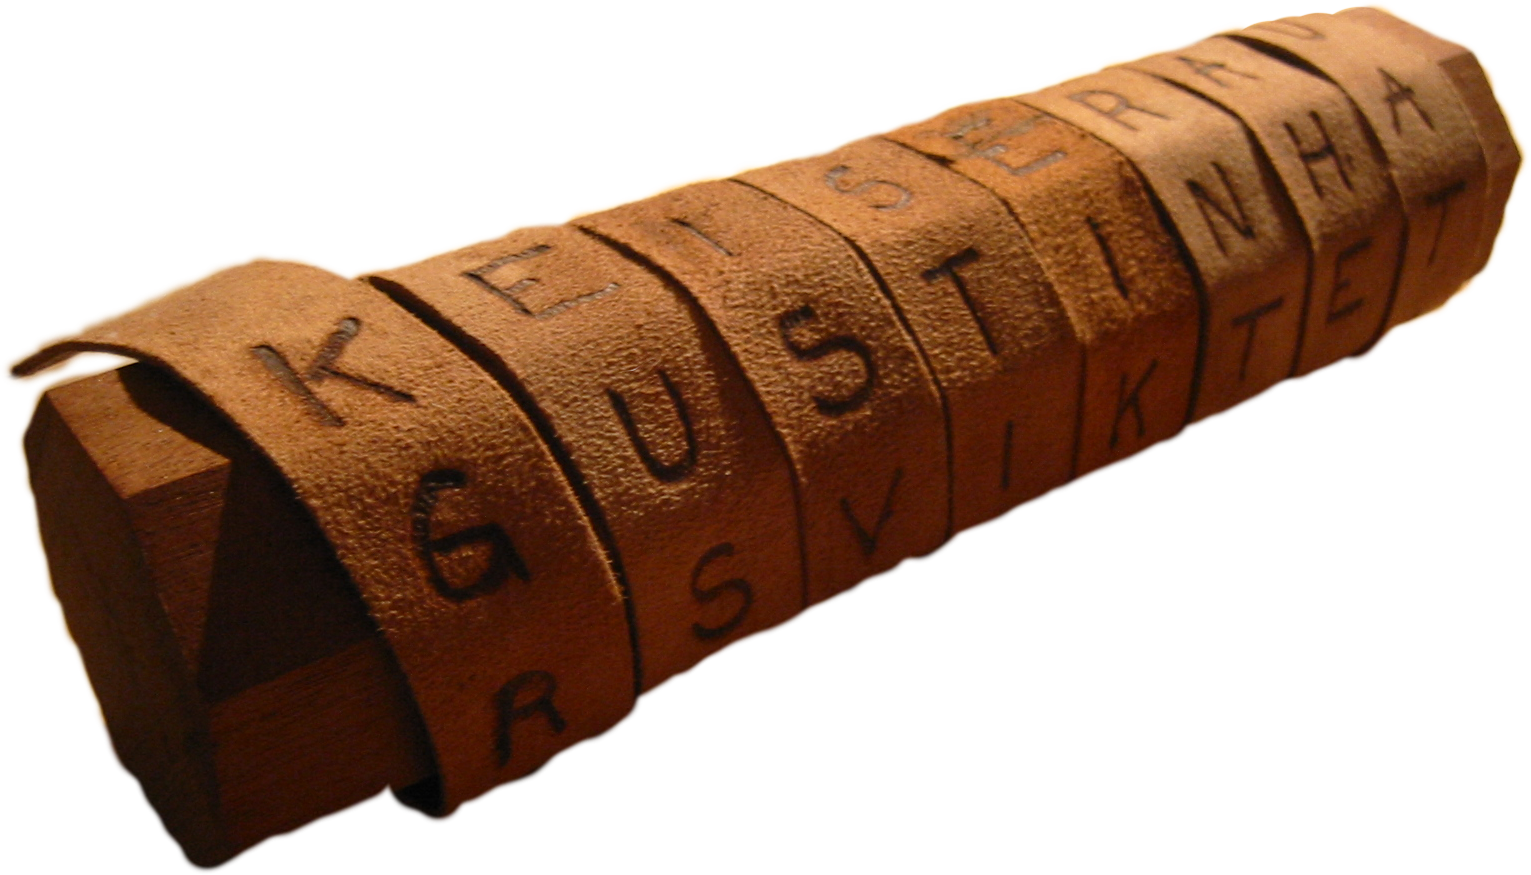
\includegraphics[width=\marginparwidth]{images/skytale}
\caption[A Scytale]{A band of parchment was first wrapped around the scytale, then the message was written one letter per convolution. Once unfolded, the message would be unreadable except for the receiver which would have another scytale of the same diameter. }
\label{fig:scytale}
}

Caesar's cypher may be one of the simplest cryptographic technique.
In this technique, letters are replaced by another letter at a given distance in the alphabet.
Julius Caesar was reported as using this cypher with a shift of three letter to write secret messages to his generals.
Knowing the shift value, \ie the secret key, a recipient of an encrypted message could reverse the shift to uncover the plaintext message.
Alberti invented around 1467 a polyalphabetic substitution cypher where the key is modified at random through the text.
Though later works derive from Alberti's invention, such cryptography technique was already known by the 8th century's mathematician Al-Kindi.
Substitution cyphers are vulnerable to letter frequency attack.
Indeed, a cryptanalyst can guess the key of a simple substitution cypher by comparing the letter frequencies of the cyphertext to the letter frequencies of another plaintext known to be written in the same language.
Polyalphabetical substitutions try to alter the frequency of letters by continuously changing the substitution alphabet.
These are however still vulnerable to more complex frequency analysis.
The development of substitution cyphers was thus a race between cryptographers inventing new keying mechanisms and cryptanalysts.

Rotor machines, such as the famous Enigma machine, brought a large increase in the number of possible substitutions. 
Cryptanalysis efforts by allied researchers during the second world war resulted in the development of the first programmable computer.
This breakthrough also allowed the use of much more complex cyphers based on complex mathematical problems.
Furthermore, computers allow the encryption of any kind of data encoded as a sequence of bits.
The development of computer and public cryptographic algorithms made security accessible to small companies and individuals. 
Everyday communications are now encrypted by default, and users are being educated to pay attention to security indications~\cite{mozillasecurityblog2017communicating} such as the one presented in Figure~\ref{fig:firefox_warning}.
This, however, does not solve every issue: a trusted third party is still often required to set up the communication.

\marginpar{
\captionsetup{type=figure}
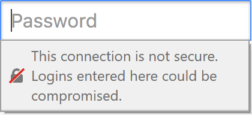
\includegraphics[width=\marginparwidth]{images/firefox_warning}\\\\
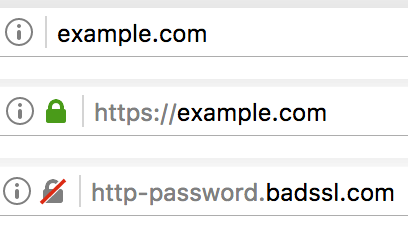
\includegraphics[width=\marginparwidth]{images/httpslevel}
\caption[Browser Security Indications]{By displaying warning on insecure HTTP webpage, the Firefox web browser is educating its users to the faced risk, and at the same time pushing web developers to implement security for HTTP.}
\label{fig:firefox_warning}
}

%% TRUST DEFINITION

Several definitions of trust have been proposed.
Inspired by McKnight and Chervany~\cite{mcknight1996meanings}, J{\o}sang and Presti define trust as: ``the extent to which one party is willing to depend on something or somebody in a given situation with a feeling of relative security, even though negative consequences are possible''~\cite{josang2004analysing}.
In the sense of an action, we would say that trust is the decision of intelligent agents to cooperate in the face of risk and uncertainty about the behaviour (capability or intention) of other agents.
This heuristic is often based on prior interaction history, reputation from a community or recommendations from other trusted sources.
 
%% SECURITY DEFINITION
Information security, on the other hand, aims at protecting information exchanged during a communication, by ensuring that certain security properties are met:
\begin{itemize}
\item The secrecy of the exchange, \ie the \textit{privacy}.
\item The \textit{confidentiality} of the exchanged message.
\item The \textit{integrity} of the content.
\item The \textit{non-repudiation} of the communication.
\item The \textit{authentication} of the other peer's identity.
\end{itemize}

Fully secure systems are difficult to build and may be impractical for everyday usage. 
In this situation, trust may be a more relaxed way of ensuring the security of the communication.

The World Wide Web (in short: the Web) is built on a client-server model.
Its security is based on a certificate chain anchored into the \gls{ua}, usually a web browser, acting as the \gls{tcb}.
Websites are authenticated by their certificates and communications between the \gls{ua} and the server are secured by protocols such as \gls{tls}. 
The emerging web functionalities offer a lot more possible use-cases through JavaScript web \gls{api} and \gls{http}~\cite{RFC2616} based protocols.
These new relations are often tripartite between a user and two other servers, a service provider and a \gls{rp}.
This is, for instance, the case in authentication delegation scenarios.
In these tripartite situations, each party cannot fully monitor interactions between the others parties.
The security and trustworthiness of such communication may be more difficult to assess.
As a result, it is up to each entity to take a decision based on subjective criteria and its own evaluation of the faced risk, \ie to take a trust decision.

Real-time media and data communication is another complex use-case involving more than a single client-server relation.
On one hand, legacy inter-operable communication systems, operated by telephony companies and Internet service providers (often referred as Telco) have been cluttered by issue regarding the trustworthiness of their incoming call.
These legacy services suffer from a weak trust and identity model which is subject to abuse.
The openness of trust-circle networks and the availability of computation power allow malicious actors to launch thousands of robocalls at once\footnote{In 2014, the United States' Federal Trade Commission has received over 22 million complaints about illegal and unwanted phone calls~\cite{tu2016sok}.
Even though the practice of phone spam is illegal in the European Union without an opt-in from the recipient, in France 1,6 million voice and SMS spams were reported in 2016 to the 33700, the national spam reporting number~\cite{33700}.}.
This factor could be one of the reasons behind the drop of value in telephony services~\cite{arcep_observatoire}, a major asset of Telco, benefiting to \gls{ott}\footnote{\gls{ott} services are provided on top of existing internet service providers networks} services.
On the other hand, \gls{ott} are rapidly gaining market share over Telco but are all set in silo model.
The silo model implies that while these services benefit from a controlled trust model, they cannot communicate with each other and are the theatre of an intensive battle to become, or stay, the hegemonic service\footnote{Chocking examples of this competition were the buyout of Whatsapp and its 450 millions users in 2014 by Facebook for \$16 billions~\cite{goel_facebook}, and the buyout of Skype and its 663 millions users by Microsoft in 2011~\cite{rosoff_microsoft}. In particular, the Skype buyout was conducted after rumours of interest from Cisco, Google, and Facebook, \ie Microsoft's competitors.}.
As it is difficult to change network without losing the ability to reach their contacts, users are de-facto captive of these services.

WebRTC is a set of web \gls{api} and protocols, specified by the \gls{w3c} and the \gls{ietf}, which supports \gls{p2p} audio-video calling and data sharing.
As WebRTC brings useful new functionalities to the web ecosystem, its deployment could be an opportunity to open the future \gls{ott} services.
For the WebRTC specification to succeed, it should learn from the issues encountered by previous technologies.
As past experiences have proved~\cite{RFC5039}, a weak identity model may have an important impact later on and is particularly hard to fix once the system is deployed.

\section*{A Motivating Scenario}
\label{introduction.scenario}
%Currently the main WebRTC use case is to easily integrate real-time communication into a webpage.
In a conference call, several users connect to a single room to organise a meeting.
Users share their audio and video, they may also share some documents or their screen~\cite{w3c:screencapture}.
%WebRTC is particularly fitting to this use case due to the possibility to open media and data channels.
%Technically, sessions between users may be organised in a mesh topology, but more realistically an efficient architecture would use a Multipoint Control Unit. 
Several communication services are already offering this kind of service, some using WebRTC. 
However, a common issue appears when participants connect from different company, for instance during a collaborative project.
While the service is often integrated with one company's \gls{idp}, participants from other companies may not authenticate with it and may have to fallback to a declarative or self-asserted identity.
Because the subject of their conversation is sensible, participants want to ensure that no one is maliciously listening, including the communication service itself which may come from a third party company.
Currently, implementation decisions made by the \gls{cs} website drastically limit the user's choice.
And at the same time communication services are missing the capability to interface with any \gls{idp}.

Going further, supposing every participant authenticated to each other, one of them may want to raise the security level of the session.
Each participant would then be required to authenticate with a higher strength, and the session security would be renegotiated with stronger parameters.
For this to be possible, it is required to have a model of the trust and security level of the session and a mechanism to negotiate it.
In the long-term, the future telephony will move to a fully IP-based network, interconnected with the Web.
In this scenario, inter-operability, \ie the ability for a user of one \gls{cs} to call a user from another \gls{cs}, could be imposed by regulations.
Some projects are already writing work in progress inter-operable \gls{cs} architectures~\cite{toutain2015webco,matrix,rethink}.
Evaluating the security of a call session is necessary for users to make an informed trust decision on whether or not to accept or pass a call.
However, in these inter-operable architectures, the communication stack is drastically more complex than the usual client-server model.

\section*{Open Challenges}
\label{introduction.challenges}
Our intuition is that users should be given more information and control over the security and trust level of their communications.
This is our global objective.
For this to be possible, we need to build a model that could represent the communication setup, the different channels, protocols, and the actors in operation.
This model would allow us to forge a single metric characterising the risk of using the communication system, \ie the trust and security level.
It would also be a useful tool to model an instance of a communication setup specification and discuss it with expert.

To inform the user of the security of its communication session, it is necessary to answer the following questions:
\begin{itemize}
\item How to model the security of a communication setup made with several distinct channels, protocols, and actors?
\item Can the same model integrate trust and security information into a single meaningful metric?
\item Which parameters of the communication setup can be used to forge this metric?
\item Can we build this model at runtime?
\end{itemize}

Supposing we dispose of a trust and security model for the communication setup, we could leverage this model to raise the trust and security level of the session.
This process could either be manually or automatically controlled by the user.
To give this kind of control to the users, we would also have to answer the following questions:
\begin{itemize}
\item Can users control and eventually raise the trust and security level of their communication sessions?
\item Is it possible to trust a communication setup in which some of the actors are not trusted?
\item Can users choose trusted actors to participate in their communication setup?
\end{itemize}

As we mentionned, legacy communication services obey strict standards allowing interoperability between actors.
%There may be several actors on the network, but they operate under the same configurations.
There are also multiple \gls{ott} communication services, but since they are set in silo and often operate closed-source softwares, we consider them as blackboxes.
WebRTC, however, is a disruptive technology for web real-time communications.
It is envisioned, given the simplicity to deploy a WebRTC service, that the number of WebRTC enabled websites could skyrocket in the near future.
Considering the proposed use cases, the number of WebRTC services, and the other actors: the complexity of communication setup, from a trust and security perspective, could be difficult to assess for non-expert users.
At the moment, WebRTC's final version of the specification has not yet been published, and some functionalities are yet to be implemented in web Browsers\footnote{The state of WebRTC implementations on web browsers can be followed on Mozilla's developer website: \url{https://developer.mozilla.org/en-US/docs/Web/API/RTCPeerConnection}.}.
It may be the right time to challenge its security architecture.

For these reasons, we want to address our research questions with respect to the WebRTC specifications.
We want to understand to which extent users could trust a WebRTC session, even if some parties are untrusted.
Our first research question is thus the following:

\begin{itemize}
\item \textbf{RQ1}: What are the risks for the user of a WebRTC session and which abstractions can we use to show these risks to the user?
\end{itemize}

One way to ensure that the session is secured is to interact with trusted parties, either before the session is established, or during the session to raise the trust level.
This opens the two following questions:
\begin{itemize}
\item \textbf{RQ2}: Can we act on a WebRTC session to raise the trust and security level? 
\item \textbf{RQ3}: Can we let users chose actors they trust to participate in the communication setup?
\end{itemize}

\section*{Contributions}
\label{introduction.contributions}
In this thesis, I propose three main contributions:

In our first contribution, we study the WebRTC identity architecture and more particularly its integration with existing authentication delegation protocols.
This integration has not been studied yet. 
To fill this gap, we implement components of the WebRTC identity architecture and comment on the issues encountered in the process.
In order to answer RQ1, we then study this specification from a privacy perspective and identify new privacy considerations related to the central position of \gls{idp}.
In the Web, the norm is the siloed architecture of which users are captive.
That is all the more the case for authentication delegation systems where most of the time it is not possible to freely choose an \gls{idp}.
In order to answer RQ3, we conduct a survey of the top 500 websites according to Alexa\footnote{\url{https://alexa.com}} to identify the reasons why users cannot choose their \gls{idp}.

In our second contribution, we aim at giving more control to users.
To this end and in order to answer RQ2, we extend the WebRTC specification to allow identity parameters negotiation.
We present a prototype implementation of our proposition to validate our proposition.
We then propose a web \gls{api} allowing users to choose their \gls{idp} in order to authenticate on a third-party website.
Our \gls{api} reuse components of the WebRTC identity architecture in a client-server authentication scenario. 
Again, we validate our proposition by presenting a prototype implementation of our \gls{api} based on a Firefox extension.

Finally, in our third contribution, we look back on RQ1 and propose a trust and security model of a WebRTC session.
Our proposed model integrates into a unique metric the security parameters used in the session establishment, the encryption parameters for the media streams, and trust in actors of the communication setup as defined by the user.
Our model's objective is to help non-expert users to better understand the security of their WebRTC session.
To validate our approach, we conduct a preliminary study on the comprehension of our model by non-expert users.
This study is based on a web survey offering users to interact with a dynamic implementation of our model.

Figure~\ref{contrib} represents how our contributions articulate and how they relate to our research questions.
In our first contribution we study the WebRTC identity architecture.
We then experiment on how to control this identity architecture to increase trust and security.
Finally and based on our knowledge, we close the loop and propose a model of the trust and security of the WebRTC security architecture.
 
\begin{figure}[H]
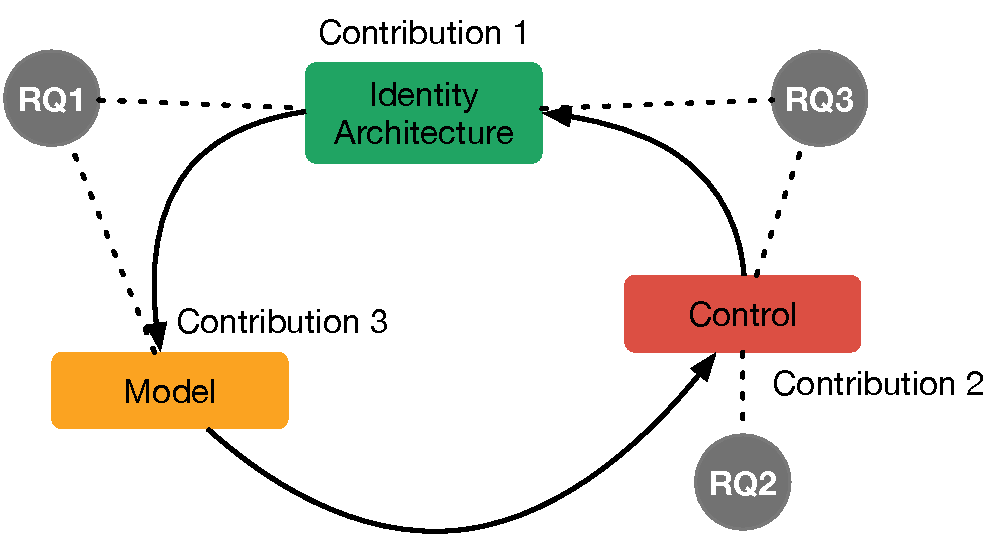
\includegraphics[scale=.5]{images/controlloop}
\caption{Overview of our Contributions}
\label{contrib}
\end{figure}


%
%\begin{figure}[tbp]
%\begin{center}
%    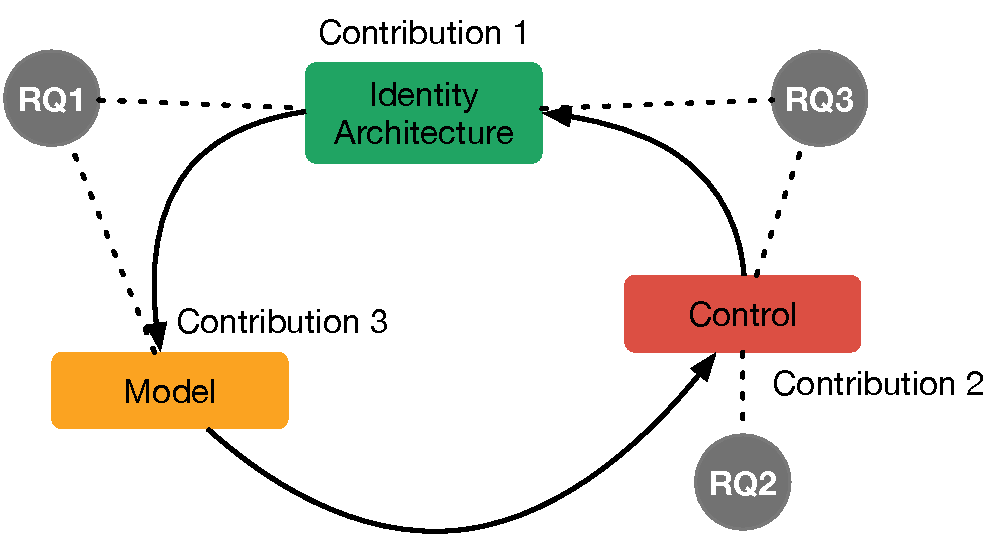
\includegraphics[width=\linewidth]{images/controlloop}
%\end{center}
%    \begin{tikzpicture}
%    \node(rq1)[rectangle, minimum width=0.6cm, minimum height=0.4cm, fill=matgreen] at (-1,0) {};
%    \node[] at (-.1,0) {\footnotesize RQ1};
%    \node(rq2)[rectangle, minimum width=0.6cm, minimum height=0.4cm, fill=matred] at (-1,-.5) {};
%    \node[] at (-.1,-.5) {\footnotesize RQ2};
%    \node(rq3)[rectangle, minimum width=0.6cm, minimum height=0.4cm, fill=matblue] at (-1,-1) {};
%    \node[] at (-.1,-1) {\footnotesize RQ3};
%    \node[] at (8,0) {};
%    \end{tikzpicture}
%\caption{Trust and security level control loop and related research questions.}
%\label{fig_controlloop}
%\end{figure}
%
%A way to represent our research questions and contributions is a control loop for the trust and security level of a WebRTC session, as present in Figure~\ref{fig_controlloop}.
%The goal of RQ1 is to build a sensor and a model, together capable of measuring the trust and security level of the session.
%In RQ2 we search to act on the session to raise the security level.
%Finally, in RQ3 we try to determine if and how users could choose trusted actors, in order to raise the trust level of the communication setup.
%

\section*{Organisation}
\label{introduction.organisation}
The document is organised in three main parts.
In the first part, we expose the context of our research.
In Chapter~\ref{security}, we detail the technical specifications used in our work such as OAuth~2 and WebRTC.
We then present the state of the art to which our work contributes in Chapter~\ref{sota}.
In the second part of this thesis, we present our contributions.
In Chapter~\ref{webrtcprivacy} we study WebRTC privacy issues based on actual implementations of the WebRTC identity architecture.
In Chapter~\ref{identitynegotiation} we propose to give users more control over their WebRTC identity parameters.
Chapter~\ref{webrtcmodel} presents a trust and security model of a WebRTC session intended to help advanced users in understanding the security of their WebRTC session.
Finally, the third part of this thesis proposes a summary of our contributions in Chapter~\ref{conclusion} and discusses our perspectives in Chapter~\ref{perspectives}.

\subsection*{Part \ref{context}:  Context}
\paragraph{Chapter \ref{security}} \textit{WebRTC Trust and Security Architecture} is an introduction to the techniques, algorithms, and protocols securing WebRTC and forming the context of our thesis.
In this chapter, we introduce the WebRTC architecture and specifications, present an overview of the concepts accomplishing practical security on the Web, and focus on the protocols used to secure a WebRTC communication.
We also introduce the concept of trust and we explain privacy in the context of the Web and in particular the privacy consideration of the WebRTC specification.
Finally, we present some signalling architecture that could be deployed by WebRTC services.

\paragraph{Chapter \ref{sota}} \textit{State of the Art} presents the state of the art on \gls{voip} security research.
We review the results of a comprehensive survey of 245 articles on \gls{voip} security and published in 2012.
As the first draft of the WebRTC specification was published the same year, this survey is a solid starting point to study the field of WebRTC security.
We then present our own survey of \gls{voip} and WebRTC security research collecting papers published between 2012 and 2017.
Based on our findings, we review collected papers dealing specifically with WebRTC.


\subsection*{Part \ref{contributions}: Contributions}
\paragraph{Chapter \ref{webrtcprivacy}} \textit{Privacy Implications of the WebRTC Identity Architecture} studies the WebRTC identity architecture from a privacy point-of-view.
The specification lacks support and, to the best of our knowledge, there is no public implementation.
We first describe our implementation of the WebRTC identity architecture and its integration with existing authentication delegation protocols.
We then comment on encountered issues and detail additional privacy considerations.
Finally, we report on our study on why users cannot choose their \gls{idp} on the Web. 


\paragraph{Chapter \ref{identitynegotiation}} \textit{Controlling the WebRTC Identity Parameters} proposes to give users more control over WebRTC identity parameters.
Firstly, we define a \gls{sdp} extension to negotiate the other peer's \gls{idp} and authentication strength during the call setup and present our implementation.
Secondly, this chapter presents WebConnect, a prototype for an Identity Metasystem \gls{api} based on the WebRTC identity specification which allows users to preserve their privacy by selecting trusted \gls{idp}.
The WebRTC identity specification offers some interesting concepts limited to the scope of user-to-user authentication, WebConnect extends them to the use case of user-to-server authentication.


\paragraph{Chapter \ref{webrtcmodel}} \textit{WebRTC Trust and Security Model} presents a trust and security model intended to help advanced users in understanding the security of their WebRTC session.
We first present our methodology to build our model and then details our actual WebRTC trust and security model.
The model evaluates security with regards to the risk presented on the confidentiality and integrity of the communication and shows which trust relations must be valid for the security level to be trusted too. 
In order to validate our approach, we present a preliminary study on the understanding of our model by advanced users based on a survey and a dynamic implementation of our model.


\subsection*{Part \ref{summary}: Conclusion and Perspectives}
\paragraph{Chapter \ref{conclusion}} \textit{Conclusion} presents the conclusions of our work.

\paragraph{Chapter \ref{perspectives}} \textit{Perspectives} discusses possible future research directions and perspectives. 
More particularly, we look at continuing work on our WebRTC trust and security model, improving the WebRTC identity architecture and integrating it with other authentication protocols, and comparing the WebRTC identity architecture to the current work of the \gls{w3c} WebPayment working group.

\section*{List of Publications}

\subsection*{Scientific Publications}
\begin{description}
\item \cite{corre_webrtc_2017} \fullcite{corre_webrtc_2017}
\item \cite{corre_whyusers_2017} \fullcite{corre_whyusers_2017}
\item \cite{javed_cross-domain_2017} \fullcite{javed_cross-domain_2017}
\end{description}

\subsection*{Internet Drafts}
\begin{description}
\item \cite{I-D.copeland-rtcweb-p2p-idp-auth} \fullcite{I-D.copeland-rtcweb-p2p-idp-auth}
\end{description}

\paragraph{A note on \gls{rfc}}: \gls{rfc} are documents published by the \gls{ietf} and describing technical aspects of the internet.
\gls{rfc} are first proposed as \textit{draft} with an expiration date of 6 months, which can be extended by submitting new version of the draft.
If an interest emerges, a working group may form.
This working group will develop the draft further until a request to publish it as a \gls{rfc} is submitted.
Not all \gls{rfc} are however submitted on the standard track.
Their status may alternatively be \textit{informational}, \textit{experimental}, \textit{best current practice}, \textit{historic}, or \textit{unknown}.

\subsection*{Patents}
\begin{description}
\item \cite{corre_authent} \fullcite{corre_authent}
\end{description}

\subsection*{Technical Reports}
\begin{description}
\item \cite{copeland_framework_2015} \fullcite{copeland_framework_2015}

\item \cite{crom_management_2015} \fullcite{crom_management_2015}

\item \cite{crom_implementation_2016} \fullcite{crom_implementation_2016}

\item \cite{crom_implementation_2017} \fullcite{crom_implementation_2017}

\end{description}



\section*{}
This thesis presents the results of my three years research work. 
It is the result of a collaboration between the Identity and Trust Architecture research project from Orange Labs and the INRIA DiverSE Team.
We also contributed to the H2020 reThink project for its identity and security architecture. 